\PassOptionsToPackage{sort&compress}{natbib}
\documentclass[preprint]{elsarticle}

% \usepackage{natbib} not needed. Already added by elsarticle
\setcitestyle{numbers,round}

% To remove square brackets from reference list
\makeatletter 
\renewcommand\@biblabel[1]{#1} 
\makeatother

\usepackage{lineno,hyperref}
\modulolinenumbers[1]

% For equations
\usepackage{amsmath}
\usepackage{amssymb}

% Highlight
\usepackage{soul,xcolor}

% For the table
\usepackage{booktabs}
\usepackage{geometry}
\usepackage{array}

% To add notes to margins
\usepackage[colorinlistoftodos]{todonotes}

% To force figure position
\usepackage{float}

% To striketrough
\usepackage[normalem]{ulem}

\journal{Aperture}

%%%%%%%%%%%%%%%%%%%%%%%
%% Elsevier bibliography styles
%%%%%%%%%%%%%%%%%%%%%%%
%% To change the style, put a % in front of the second line of the current style
%and % remove the % from the second line of the style you would like to use.
%%%%%%%%%%%%%%%%%%%%%%%

%% Numbered \bibliographystyle{model1-num-names}

%% Numbered without titles \bibliographystyle{model1a-num-names}

%% Harvard
% \bibliographystyle{model2-names.bst}\biboptions{authoryear}

%% Vancouver numbered
%\usepackage{numcompress}\bibliographystyle{model3-num-names}
\bibliographystyle{vancouver}

%% Vancouver name/year
%\usepackage{numcompress}\bibliographystyle{model4-names}\biboptions{authoryear}

%% APA style \bibliographystyle{model5-names}\biboptions{authoryear}

%% AMA style \usepackage{numcompress}\bibliographystyle{model6-num-names}

%% `Elsevier LaTeX' style \bibliographystyle{elsarticle-num}
%%%%%%%%%%%%%%%%%%%%%%%

\begin{document}

\begin{frontmatter}

\title{Hemodynamic Deconvolution Demystified: Sparsity-Driven Regularization at Work}

%% Group authors per affiliation:
\author[bcbl,upv]{Eneko Uru\~nuela\corref{mycorrespondingauthor}}
\cortext[mycorrespondingauthor]{Corresponding authors}
\ead{e.urunuela@bcbl.eu}

\author[epfl,chuv]{Thomas A.W. Bolton}
\author[epfl,unige]{Dimitri Van De Ville}
\author[bcbl]{C\'{e}sar Caballero-Gaudes\corref{mycorrespondingauthor}}
\ead{c.caballero@bcbl.eu}

\address[bcbl]{Basque Center on Cognition, Brain and Language (BCBL),
Donostia-San Sebasti\'{a}n, Spain.} \address[upv]{University of the Basque
Country (EHU/UPV), Donostia-San Sebasti\'{a}n, Spain.}
\address[epfl]{Ecole Polytechnique F\'ed\'erale de Lausanne (EPFL), Lausanne, Switzerland.}
\address[chuv]{Gamma Knife Center, Department of Clinical Neuroscience, Centre Hospitalier Universitaire Vaudois (CHUV), Lausanne, Switzerland}
\address[unige]{Faculty of Medicine, University of Geneva, Geneva, Switzerland}

\begin{abstract}
Deconvolution of the hemodynamic response is an important step to access short
timescales of brain activity recorded by functional magnetic resonance imaging
(fMRI). Albeit conventional deconvolution algorithms have been around for a long
time (e.g., Wiener deconvolution), recent state-of-the-art methods based on
sparsity-pursuing regularization are attracting increasing interest to
investigate brain dynamics and connectivity with fMRI. This technical note
revisits the main concepts underlying two main methods, Paradigm Free Mapping
and Total Activation, in the most accessible way. Despite their apparent
differences in the formulation, these methods are theoretically equivalent as
they represent the synthesis and analysis sides of the same problem,
respectively. We demonstrate this equivalence in practice with their
best-available implementations using both simulations, with different
signal-to-noise ratios, and experimental fMRI data acquired during a motor task
and resting-state. We evaluate the parameter settings that lead to equivalent
results, and showcase the potential of these algorithms compared to other common
approaches. This note is useful for practitioners interested in gaining a better
understanding of state-of-the-art hemodynamic deconvolution, and aims to answer
questions that practitioners often have regarding the differences between the
two methods.
\end{abstract}

\begin{keyword}
fMRI deconvolution, paradigm free mapping, total activation, temporal
regularization
\end{keyword}

\end{frontmatter}

\linenumbers

% Introduction
\section{Introduction}

\begin{itemize}

    \item Talk about our motivation for this paper.

    \item We could mention iCAPs Neuron, and papers with applications like PFM, TA, clinical patient papers with iCAPs.

    \item Apart from [[Richard F. Betzel]]'s work~\cite{betzel2020temporal,esfahlani2020high,faskowitz2020edge}, we could mention the connection with the
    [[Multiplication of Temporal Derivatives]] method~\cite{shine2015estimation,shine2016dynamics}.

    \begin{itemize}
        \item These are basically calculating the derivative, which is the same as applying a high-pass filter and calculating the correlation.
    \end{itemize}

\end{itemize}

There is an increasing interest in methods that aim to recover the underlying neuronal activity from functional magnetic resonance imaging (fMRI) data with no prior information of the timing of the blood oxygenation level-dependent (BOLD) events. One of such techniques is deconvolution, which does not consider task-related stimulus functions or any other specific cause of the underlying neuronal activity. In other words, deconvolution methods are capable of blindly estimating the neuronal activity, which makes them especially attractive for exploring time-varying activity of resting-state fluctuations~\cite{petridou2013periods,karahanouglu2015transient,karahanouglu2017dynamics,kinany2020dynamic}, naturalistic paradigms, or clinical conditions such as the study of interictal events in epilepsy. 

% Theory
\section{Theory}

% \begin{itemize}
%     \item What is deconvolution and different formulations presented as a review.
%     \item Analysis vs synthesis
%     \begin{itemize}
%         \item TA paper but without the spatial regularization
%         \item PFM paper
%         \item In Gitelman it's an \(\mathbf{H}\) multiplied by a Fourier term.
%     \end{itemize}
%     \item Spikes and block models
% \end{itemize}

The hemodynamic response to neuronal activity can be modeled as the convolution the activity-inducing signal \(s(t)\) with the hemodynamic response function \(h(t)\) as \(x(t) = h(t) * s(t)\) (\citealt{gitelman2003ModelingRegionalPsychophysiologic}). The fMRI signal at a given voxel \(y(t)\) can then be decomposed into neuronal-related hemodynamic \(x(t)\) and noise components \(n(t)\) as:
\begin{equation}
    \label{eq:gitelman}
    y(t) = x(t) + n(t),
\end{equation}
which can be reformulated in matrix notation as \(\mathbf{y} = \mathbf{Hs} + \mathbf{n}\), where \(\mathbf{y, s} \in \mathbb{R}^N\), \(\mathbf{H} \in \mathbb{R}^{N \times N}\) is the HRF in Toeplitz matrix form, and \(N\) is the number of frames of the fMRI acquisition. The signal model in~\eqref{eq:gitelman} can also be extended to represent the neuronal signal \(\mathbf{s}\) in terms of its innovation signal \(\mathbf{u}\), i.e., its derivative, as \(\mathbf{s} = \mathbf{Lu}\) where \(\mathbf{L} \in \mathbb{R}^{N \times N}\) is an integration operator (\citealt{cherkaoui2019SparsitybasedBlindDeconvolution,urunuela2020StabilityBasedSparseParadigm}).

The maximum likelihood estimate of the hemodynamic response to the underlying neural activity can then be calculated using the ordinary least-squares estimator that minimizes the residual sum of squares between the modeled (\(\mathbf{Hs}\)) and measured (\(\mathbf{y}\)) signals. When the information about the timings of the BOLD events is known, activity maps can be obtained by solving a GLM replacing the HRF matrix \(\mathbf{H}\) with a design matrix containing the regressors with the timings. Yet, when this information is unavailable, the design matrix \(\mathbf{H}\) can be described as the Toeplitz convolution matrix with shifted HRFs (see Figure~\ref{fig:hrf_diff}B). In this case, the estimates of the neuronal activity \(\mathbf{s}\) must be constrained with a regularization term to attenuate the collinearity and high variability of the design matrix \(\mathbf{H}\), and the estimation of the underlying neural activity becomes a deconvolution problem.

%%%%%%%%%%%%%%%%%%%%%%%%%%%%%%%%%%%%%%%%%%%%%%%%%%%%%%%%%%%%%%%%%%%%%%%%
% Paradigm Free Mapping
%%%%%%%%%%%%%%%%%%%%%%%%%%%%%%%%%%%%%%%%%%%%%%%%%%%%%%%%%%%%%%%%%%%%%%%%

\subsection{Synthesis-based deconvolution}

Synthesis-based Paradigm Free Mapping (PFM) builds upon the signal model introduced in~\eqref{eq:gitelman}; i.e., the BOLD signal is the result of convolving the underlying neural activity with the hemodynamic response, and proposes to estimate the activity-inducing signal by solving the following regularized least-squares problem (\citealt{caballerogaudes2013ParadigmFreeMapping,urunuela2020StabilityBasedSparseParadigm,gaudes2011DetectionCharacterizationSingletrial}):
\begin{equation}
    \label{eq:pfm}
    \hat{\mathbf{s}} = \arg \min_{\mathbf{s}} \frac{1}{2} \| \mathbf{y} - \mathbf{Hs} \|_2^2 + \Omega(\mathbf{s}),
\end{equation}
where \(\Omega(\mathbf{s})\) is the regularization term.

Assuming that single-trial BOLD responses are the result of brief bursts of neuronal activation, the activity-inducing signal \(\mathbf{s}\) must be a sparse vector. Thus, sparse estimates of \(\mathbf{s}\) could be obtained by substituting \(\Omega(\mathbf{s})\) in~\eqref{eq:pfm_spike} with an \(l_0\)-norm and solving the optimization problem (\citealt{bruckstein2009SparseSolutionsSystems}). However, due to the convolution model defined in~\eqref{eq:pfm_spike}, finding the optimal solution to the problem demands an exhaustive search across all possible combinations of the columns of the design matrix \(\mathbf{H}\). Hence, a pragmatic solution is to solve the optimization problem with the use of an \(l_1\)-norm, or LASSO (\citealt{tibshirani1996RegressionShrinkageSelection}), which is a convex function and therefore provides fast convergence to the optimal solution.
\begin{equation}
    \label{eq:pfm_spike}
    \hat{\mathbf{s}} = \arg \min_{\mathbf{s}} \frac{1}{2} \| \mathbf{y} - \mathbf{Hs} \|_2^2 + \lambda \| \mathbf{s} \|_1,
\end{equation}
where \(\lambda\) regulates how sparse the optimal solution is.

Such formulation provides flexibility to expand the capabilities of PFM. For instance, incorporating the integration operator \(\mathbf{L}\) into the design matrix \(\mathbf{H}\) allows the recovery of the innovation signal \(\mathbf{u}\); i.e., the derivative of the activity-inducing signal \(\mathbf{s}\). Therefore, the innovation signal can be estimated by solving the following optimization problem (\citealt{cherkaoui2019SparsitybasedBlindDeconvolution,urunuela2020StabilityBasedSparseParadigm}):
\begin{equation}
    \label{eq:pfm_block}
    \hat{\mathbf{u}} = \arg \min_{\mathbf{u}} \frac{1}{2} \| \mathbf{y} - \mathbf{HLu} \|_2^2 + \lambda \| \mathbf{u} \|_1.
\end{equation}

%%%%%%%%%%%%%%%%%%%%%%%%%%%%%%%%%%%%%%%%%%%%%%%%%%%%%%%%%%%%%%%%%%%%%%%%
% Total Activation
%%%%%%%%%%%%%%%%%%%%%%%%%%%%%%%%%%%%%%%%%%%%%%%%%%%%%%%%%%%%%%%%%%%%%%%%

\subsection{Analysis-based deconvolution}

Even though based on the same signal model as PFM, analysis-based Total Activation (TA) proposes to use a linear differential operator \(L_h\) that inverts the hemodynamic system based on activelets to recover the activity-inducing signal \(\mathbf{s}\) (\citealt{karahanoglu2013TotalActivationFMRI,khalidov2011activelets,karahanoglu2011SignalProcessingApproacha}):
\begin{equation}
    L_h\{x\}(t) = s(t)
\end{equation}
where \(x\) is the neuronal-related signal; i.e., the activity inducing signal \(\mathbf{s}\) convolved with the HRF, and \(L_h\) is defined as
\begin{equation}
    L_h\ = \prod_{i=1}^{M_1} (D-\alpha_i I) (\prod_{j=1}^{M_2} (D - \gamma_j I))^{-1},
\end{equation}
where \(D\) is the derivative operator, \(\alpha_i (i=1, \hdots, M_1)\) define the zeros of the filter, \(\gamma_j (j=1, \hdots, M_2)\) represent the poles, \(I\) is the identity matrix and \(M_1 > M_2\). Given the relationship between the activity-inducing and the innovation signal, the latter can be recovered as:
\begin{equation}
    L\{x\}(t) = D\{s\}(t) = u(t)
\end{equation}
where \(L = DL_h\) and \(D\) is the derivative.

Therefore, for a given voxel, the neuronal-related signal could be estimated by solving the following regularized least-squares problem:
\begin{equation}
    \hat{\mathbf{x}} = \arg \min_{\mathbf{x}} \frac{1}{2} \| \mathbf{y} - \mathbf{x} \|_2^2 + \Omega(\mathbf{x}),
\end{equation}
where \(\mathbf{y}\) is the fMRI data and \(\mathcal{R}(\mathbf{x})\) is the following \(l_1\)-norm regularization term:
\begin{equation}
    \hat{\mathbf{x}} = \arg \min_{\mathbf{x}} \frac{1}{2} \| \mathbf{y} - \mathbf{x} \|_2^2 + \lambda \| \Delta_L \{\mathbf{x}\} \|_1,
\end{equation}
where \(\lambda\) is the regularization parameter.

This work evaluates the core of the two techniques, i.e., the regularized least-squares problem with temporal regularization, which corresponds to the generalized total-variation operator in Total Activation. Thus, we do not study the impact of spatial constraints, as we assume that spatial regularization terms should perform identically on both methods.

% Methods
\section{Methods}
\label{sec:data}

\textbf{Simulations:} In order to compare the two methods while controlling for their correct performance, we simulated a 400 seconds (TR = 2 s) activity-inducing signal with five neuronal events, convolved it with the canonical HRF, and we added noise of different sources (physiological, thermal, and motion-related) with different signal-to-noise ratios (SNR = [20 dB, 10 dB, 3 dB]) that represent low, medium and high levels of noise as shown in Figure~\ref{fig:simulations}. Noise was created following the procedure in (\citealt{caballerogaudes2013ParadigmFreeMapping}) as the sum of uncorrelated Gaussian noise and sinusoidal signals to simulate a realistic noise model with thermal noise, cardiac and respiratory physiological fluctuations. We generated the sinusoidal term as
\begin{equation}
    \sum_{i=1}^{2} \frac{1}{2^{i-1}}\left(\sin \left(2 \pi f_{r, i} t+\phi_{\mathrm{r}, i}\right)+\sin \left(2 \pi f_{c, i} t+\phi_{c, i}\right)\right),
\end{equation}
with up to second-order harmonics per cardiac (\(f_{c,i}\)) and respiratory (\(f_{r,i}\)) component that were randomly generated following normal distributions with variance 0.04 and mean \(if_r\) and \(if_c\), for \(i = [1, 2]\). We set the fundamental frequencies to \(f_r = 0.3\) Hz for the respiratory component (\citealt{birn2006separating}) and \(f_c = 1.1\) Hz for the cardiac component (\citealt{shmueli2007low}). The phases of each harmonic \(\phi\) were randomly selected from a uniform distribution between \(0\) and \(2p\) radians. In order to simulate physiological noise that is proportional to the change in BOLD signal, a variable ratio between the physiological (\(\sigma_P\)) and the thermal (\(\sigma_0\)) noise was modeled as \(\sigma_P/\sigma_0 = a(tSNR)^b + c\), where \(a = 5.01 \times 10^{-6}\), \(b = 2.81\), and \(c = 0.397\). The physiological-thermal noise model was extracted following the experimental measures of the physiological-to-thermal noise ratio at 7T in Table 3 in (\citealt{triantafyllou2005comparison}).

\begin{figure}[h]
    \begin{center}
        \includegraphics[width=\columnwidth]{figures/sim.pdf}
    \end{center}
    \caption{Simulated signal with different SNRs (20 dB, 10 dB and 3 dB).}
\label{fig:simulations}
\end{figure}

\textbf{Motor task dataset:} One healthy subject was scanned in a 3T MR scanner (Siemens) as part of a larger experiment under a Basque Center on Cognition, Brain and Language Review Board-approved protocol. T2*-weighted multi-echo fMRI data was acquired with a multiband (MB) multi-echo gradient echo-planar imaging sequence (340 scans, 52 slices, Partial-Fourier = 6/8, voxel size = 2.4x2.4x3 mm\textsuperscript{3}, TR = 1.5 s, TEs = 10.6/28.69/46.78/64.87/82.96 ms, multiband factor = 4, flip angle = 70\(^o\), GRAPPA = 2).

During the fMRI acquisition, subjects performed a motor task consisting of five different movements (left-hand finger tapping, right-hand finger tapping, moving the left toes, moving the right toes and moving the tongue). These conditions were randomly intermixed every 16 seconds, and were only repeated once the entire set of stimuli were presented. Data preprocessing consisted of optimally combining the echo time datasets, detrending of up to 5\(^{th}\)-order Legendre polynomials, spatial smoothing (3 mm FWHM) and normalization to signal percentage change. For this comparison, we selected a voxel that best represented the right-hand finger-tapping paradigm based on a generalized linear model as shown in Figure~\ref{fig:finger_tapping}.

\begin{figure}[h]
    \begin{center}
        \includegraphics[width=\columnwidth]{figures/finger_tapping.pdf}
    \end{center}
    \caption{Most representative voxel of the finger-tapping task. Green blocks indicate the onsets and the duration of it.}
\label{fig:finger_tapping}
\end{figure}

\textbf{Resting-state datasets:} One healthy subject was scanned in a 3T MR scanner (Siemens) as part of a larger experiment under a Basque Center on Cognition, Brain and Language Review Board-approved protocol. Two runs of T2*-weighted fMRI data were acquired during resting-state, each with 10 min duration, with 1) a standard gradient-echo echo-planar imaging sequence (monoband) (TR = 2000 ms, TE = 29 ms, flip-angle = 78\(^o\), matrix size = 64x64, voxel size = 3x3x3 mm\textsuperscript{3}, 33 axial slices with interleaved acquisition, slice gap = 0.6 mm) and 2) a simultaneous multislice gradient-echo echo-planar imaging sequence (multiband factor = 3) developed by the Center of Magnetic Resonance Research (University of Minnesota, USA; TR = 800 ms, TE = 29 ms, flip-angle = 60\(^o\), matrix size = 64×64, voxel size = 3x3x3 mm\textsuperscript{3}, 42 axial slices with interleaved acquisition, no slice gap). Single-band reference images were also collected in both resting-state acquisitions for head motion realignment.

During both acquisitions, participants were instructed to keep their eyes open, fixating a white cross that they saw through a mirror located on the head coil, and not to think about anything specific. Field maps were also obtained to correct for field distortions.

% Results
\section{Results}

\begin{itemize}
    \item Methods on how we're doing simulations and results (with simulations and experimental data)
    \begin{itemize}
        \item Different SNRs and maybe even use CAPs
        \item Selection of HRF explained if both use the same but it's different from what's used for simulating.
        \begin{itemize}
            \item What happens? For example with gamma for simulating.
        \end{itemize}
        \item Selection of regularization parameter
        \begin{itemize}
            \item Present with real data on a voxel
        \end{itemize}
    \end{itemize}
\end{itemize}

With the aim of making a fair comparison of the two methods, we first compared their hemodynamic response functions. Figure~\ref{fig:hrf_diff} shows the difference in the hemodynamic response function that PFM and TA use by default; the SPMG1 and the HRF resulting from the linear differential operator respectively. A clear difference is observable in that the PFM hemodynamic response function begins at zero while the TA HRF starts at 1. Hence, the Total Activation HRF starts close to its peak, which is advanced around 2.5 frames with respect to PFM. Another difference worth mentioning is that PFM normalizes its HRF to a peak amplitude of 1, whereas the TA HRF is not normalized.

\begin{figure}[h]
    \includegraphics[width=\columnwidth]{figures/hrf_diff.png}
    \caption{Diffence in the HRF of PFM (blue) and TA (orange).}
\label{fig:hrf_diff}
\end{figure}

While Paradigm Free Mapping allows for the use of any hemodynamic response function --- the columns of the design matrix \(\mathbf{H}\) are composed by shifted versions of the HRF --- the linear differential operator in TA is tailored for a fixed HRF. Hence, for practical reasons, we reproduced the HRF in the Total Activation filter and incorporated it into the PFM formulation.

\subsection{Selection of the regularization parameter based on the estimation of the noise}

\subsubsection{Simulated data}

\subsubsection{Experimental data}

\subsection{Selection of the regularization parameter by solving the regularization path}

\subsubsection{Simulated data}

\subsubsection{Experimental data}

% Discussion
\section{Discussion}

\begin{itemize}
    \item Pros and cons of each formulation: analysis vs synthesis
    \item Link with other approaches
    \item Finish with conclusions and a moving forward
    \begin{itemize}
        \item We have to refine the deconvolution
        \item HRF variability there are three: conference proceeding by Philippe~\cite{badillo2013group}, ISBI 2012 by César~\cite{gaudes2012structured}, and Farouj with a different formulation. Say conceptual differences among those.
        \item Mention stability-selection~\cite{meinshausen2010stability}
        \item Debiasing
        \item Connected to debiasing other deconvolution algorithms that are based on a norm lower than 1.
    \end{itemize}
\end{itemize}

\section{Code and data availability}
\label{sec:github}
The code and materials used in this work can be found in the following GitHub
repository: \url{https://github.com/eurunuela/pfm_vs_ta}. We encourage the
reader to explore the parameters (e.g., SNR, varying HRF options and mismatch
between algorithms, TR, number of events, onsets, and durations) in the provided
Jupyter notebooks. Likewise, the data used to produce the figures can be found
in \url{https://osf.io/f3ryg/}.

\section{Acknowledgements}
We thank Stefano Moia and Vicente Ferrer for data availability, and Younes
Farouj for valuable comments on the manuscript. This research was funded by the
Spanish Ministry of Economy and Competitiveness (RYC-2017-21845), the Basque
Government (BERC 2018-2021, PIB\_2019\_104, PRE\_2020\_2\_0227), and the Spanish
Ministry of Science, Innovation and Universities (PID2019-105520GB-100), and the
Swiss National Science Foundation (grant 205321\_163376).

\section{CRediT}
Eneko Uru\~nuela: Conceptualisation, Methodology, Software, Formal Analysis,
Investigation, Data Curation, Writing (OD), Writing (RE), Visualisation, Funding
acquisition. Thomas A.W. Bolton: Conceptualisation, Methodology, Writing (RE).
Dimitri Van de Ville: Conceptualisation, Methodology, Writing (RE). C\'{e}sar
Caballero-Gaudes: Conceptualisation, Methodology, Software, Formal Analysis,
Investigation, Data Curation, Writing (OD), Writing (RE), Visualisation, Funding
acquisition.

\bibliography{mybibfile}

\newpage
%%%%%%%%%% Merge with supplemental materials %%%%%%%%%%
\pagebreak
% \widetext
\begin{center}
\textbf{\large Supplementary Material for Hemodynamic Deconvolution Demystified: Sparsity-Driven Regularization at Work}
\end{center}
%%%%%%%%%% Merge with supplemental materials %%%%%%%%%%
%%%%%%%%%% Prefix a "S" to all equations, figures, tables and reset the counter %%%%%%%%%%
\setcounter{equation}{0}
\setcounter{figure}{0}
\setcounter{table}{0}
\setcounter{page}{1}
\makeatletter
\renewcommand{\theequation}{S\arabic{equation}}
\renewcommand{\thefigure}{S\arabic{figure}}
\renewcommand{\bibnumfmt}[1]{[S#1]}
\renewcommand{\citenumfont}[1]{S#1}
%%%%%%%%%% Prefix a "S" to all equations, figures, tables and reset the counter %%%%%%%%%%


\begin{figure*}[h!]
    \begin{center}
        \includegraphics[width=\textwidth]{figures/regpath_spike.pdf}
    \end{center}
    \caption{Spike model simulations. (Left) Heatmap of the regularization paths of the activity-inducing signal estimated with PFM and TA as a function of \(\lambda\) (increasing number of iterations in x-axis), whereas each row in the y-axis shows one time-point. Vertical lines denote iterations corresponding to the Akaike and Bayesian Information Criteria (AIC and BIC) optima. (Right) Estimated activity-inducing (blue) and activity-related (green) signals when set based on BIC. All estimates of are identical, regardless of SNR.}
\label{fig:path_spike}
\end{figure*}

\begin{figure*}[h!]
    \begin{center}
        \includegraphics[width=\textwidth]{figures/regpath_block.pdf}
    \end{center}
    \caption{Block model simulations. (Left) Heatmap of the regularization paths of the innovation signal estimated with PFM and TA as a function of \(\lambda\) (increasing number of iterations in x-axis), whereas each row in the y-axis illustrates one time-point. Vertical lines denote iterations corresponding to the Akaike and Bayesian Information Criteria (AIC and BIC) optima. (Right) Estimated innovation (blue) and activity-related (green) signals when is set based on BIC. All the estimates are identical when compared between the PFM and TA cases, regardless of SNR.}
\label{fig:path_block}
\end{figure*}

% \begin{figure*}[h!]
%     \begin{center}
%         \includegraphics[width=\textwidth]{figures/lambda_cost.pdf}
%     \end{center}
%     \caption{Lambdas and cost.}
% \label{fig:lambdas}
% \end{figure*}

\begin{figure*}[h!]
    \begin{center}
        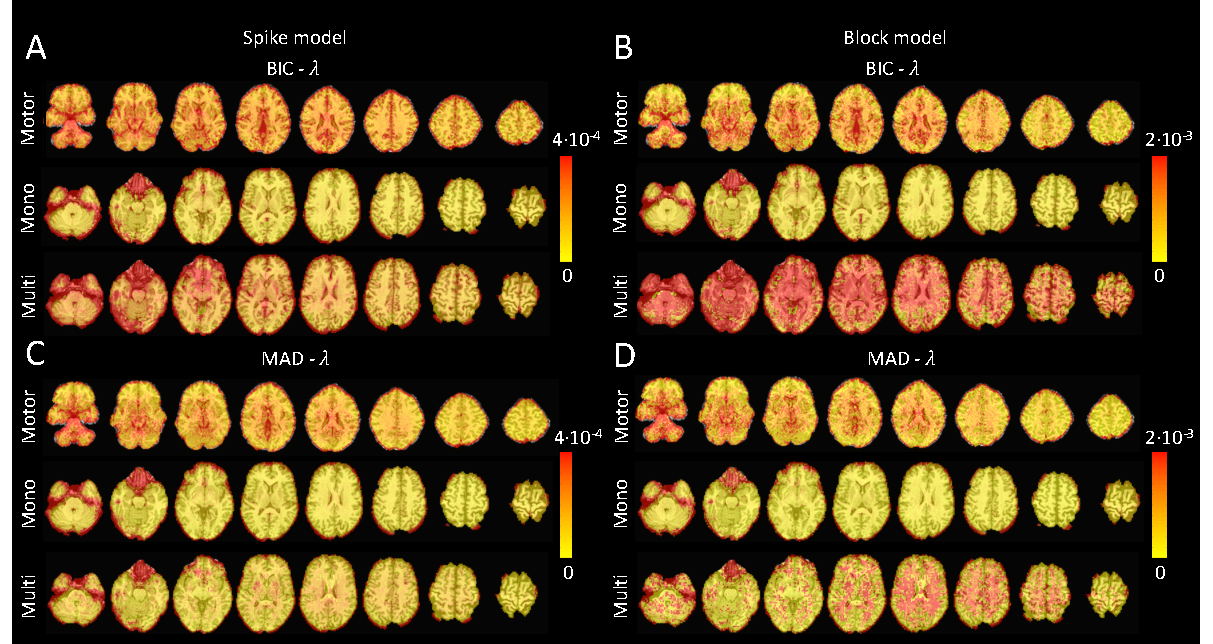
\includegraphics[width=\textwidth]{figures/supp_lambdas_map.pdf}
    \end{center}
    \caption{Lambdas.}
\label{fig:lambdas}
\end{figure*}

\begin{figure*}[h!]
    \begin{center}
        \includegraphics[width=\textwidth]{figures/supp_mad_estimate.pdf}
    \end{center}
    \caption{MAD estimate.}
\label{fig:mad_estimate}
\end{figure*}

\begin{figure*}[h!]
    \begin{center}
        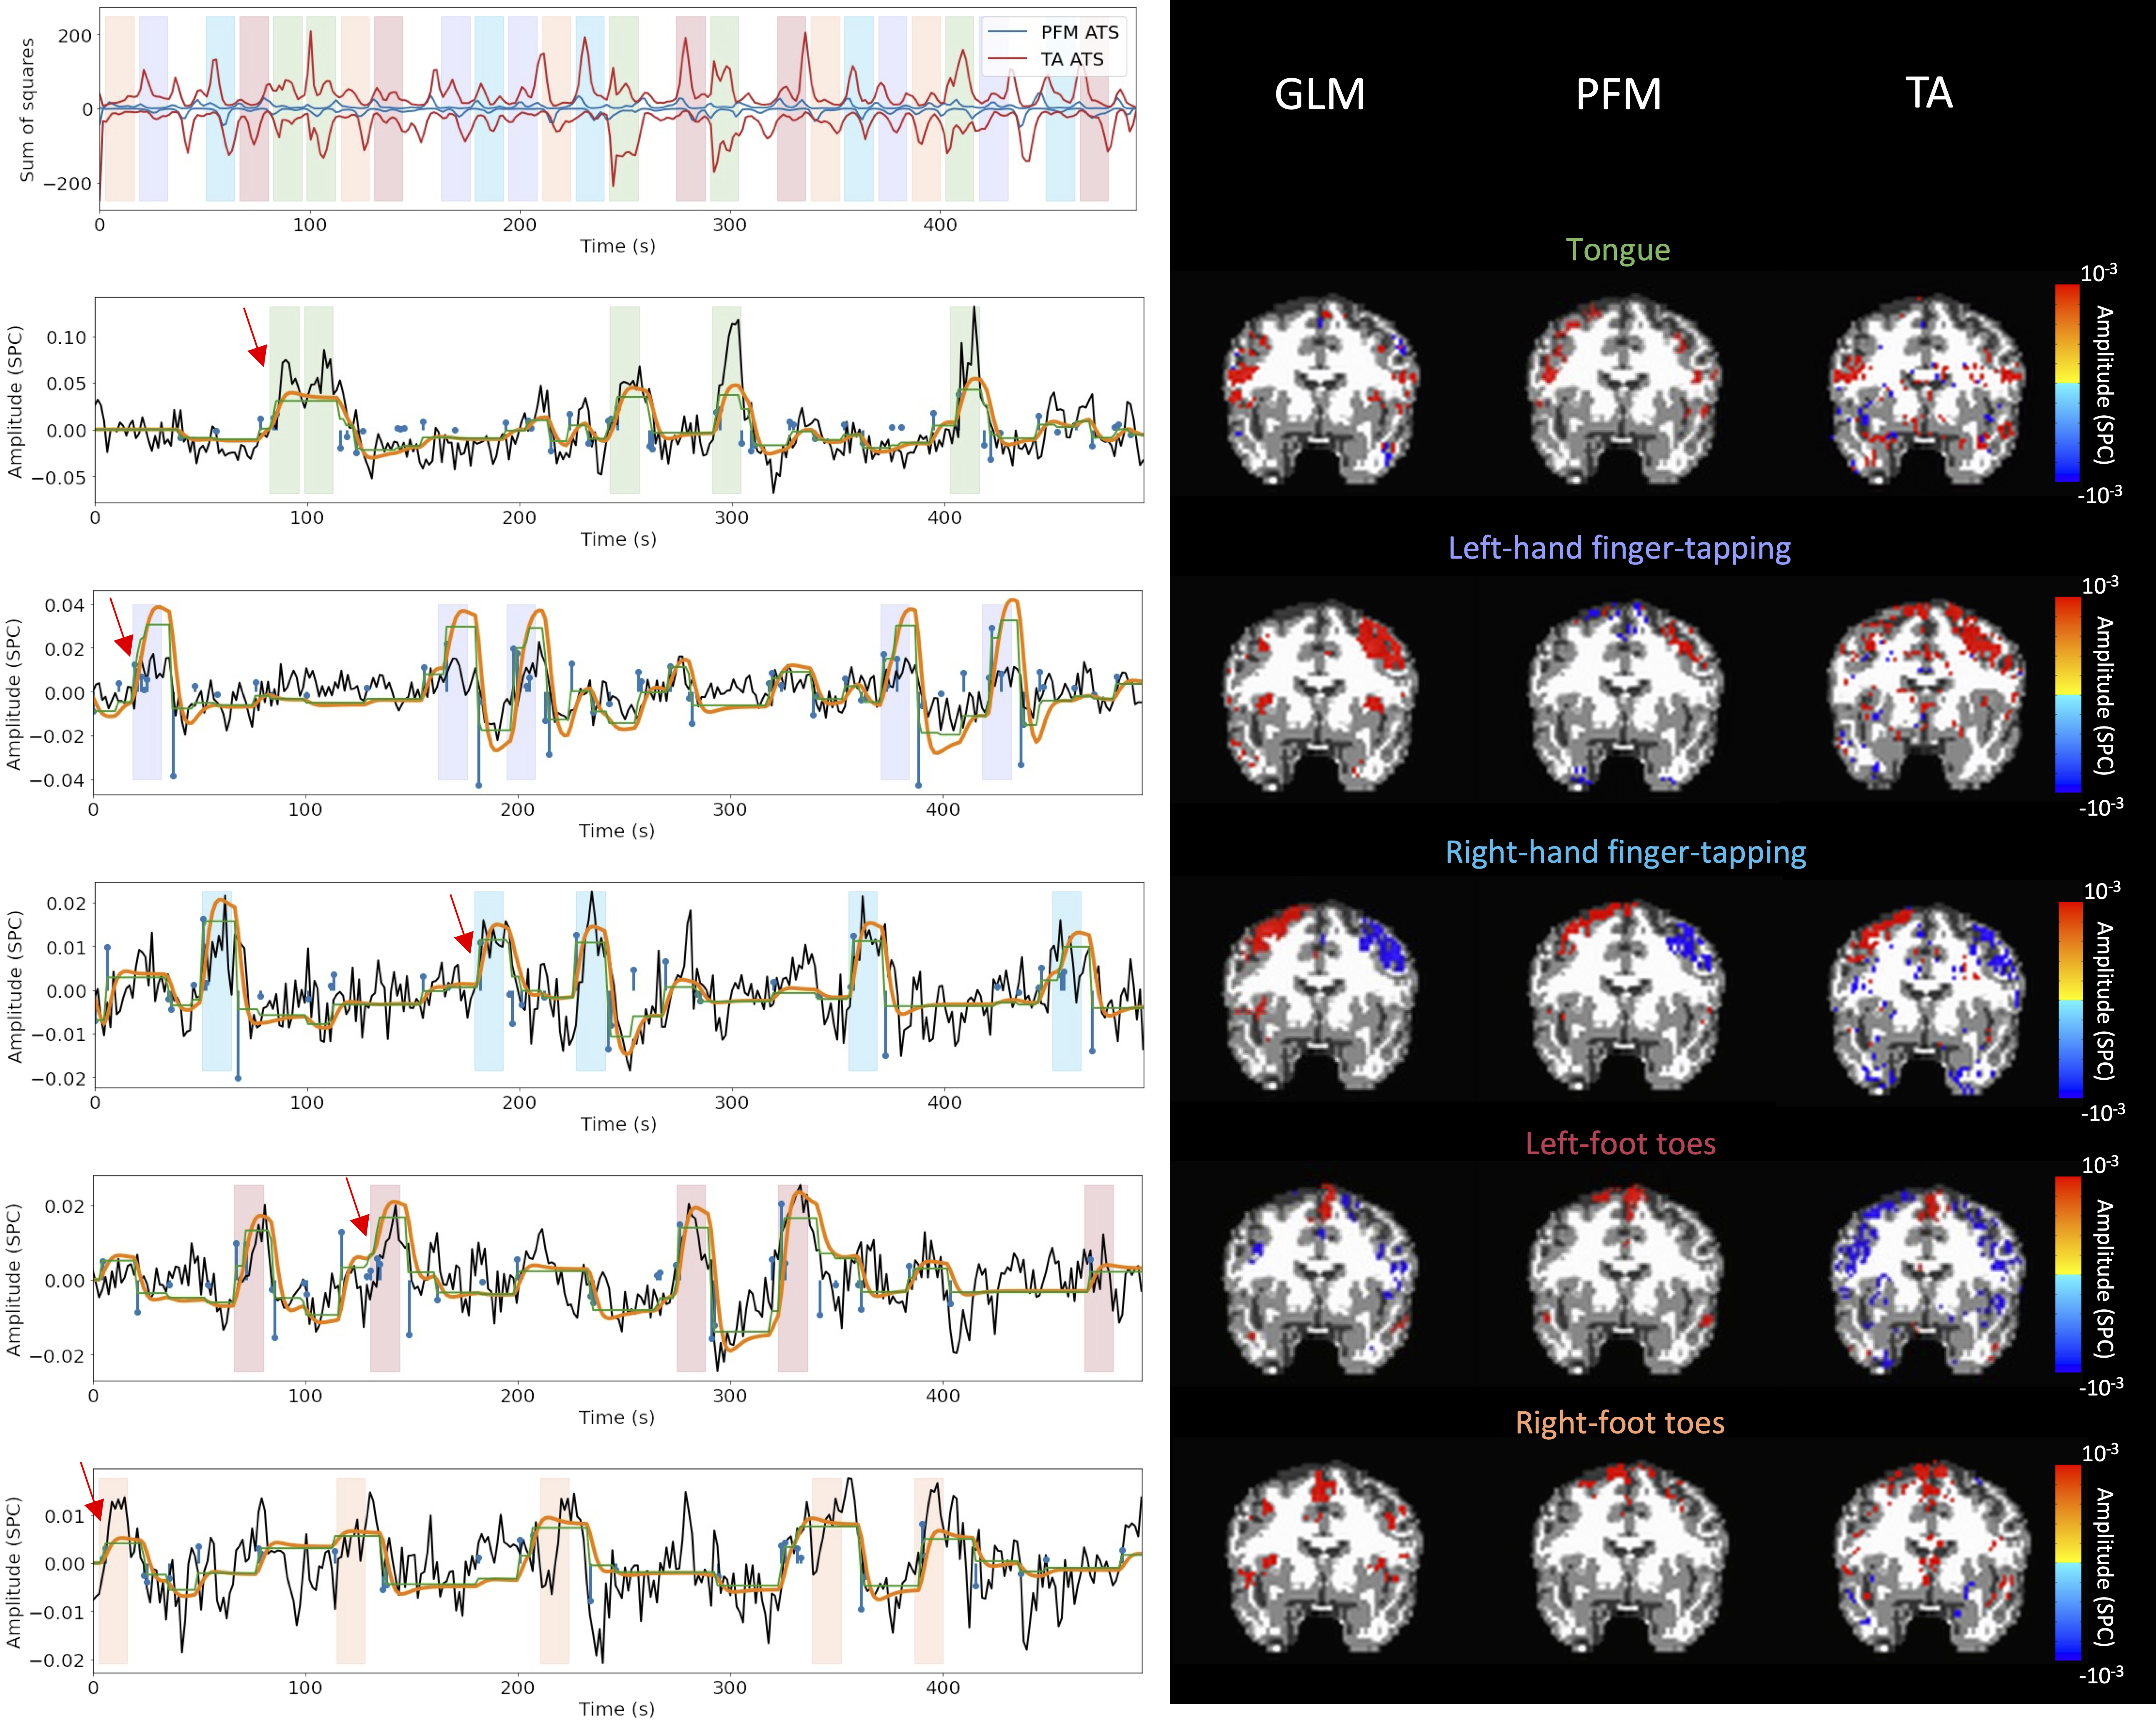
\includegraphics[width=\textwidth]{figures/supp_task_maps_mad.pdf}
    \end{center}
    \caption{Task MAD.}
\label{fig:task_mad}
\end{figure*}

\begin{figure*}[h!]
    \begin{center}
        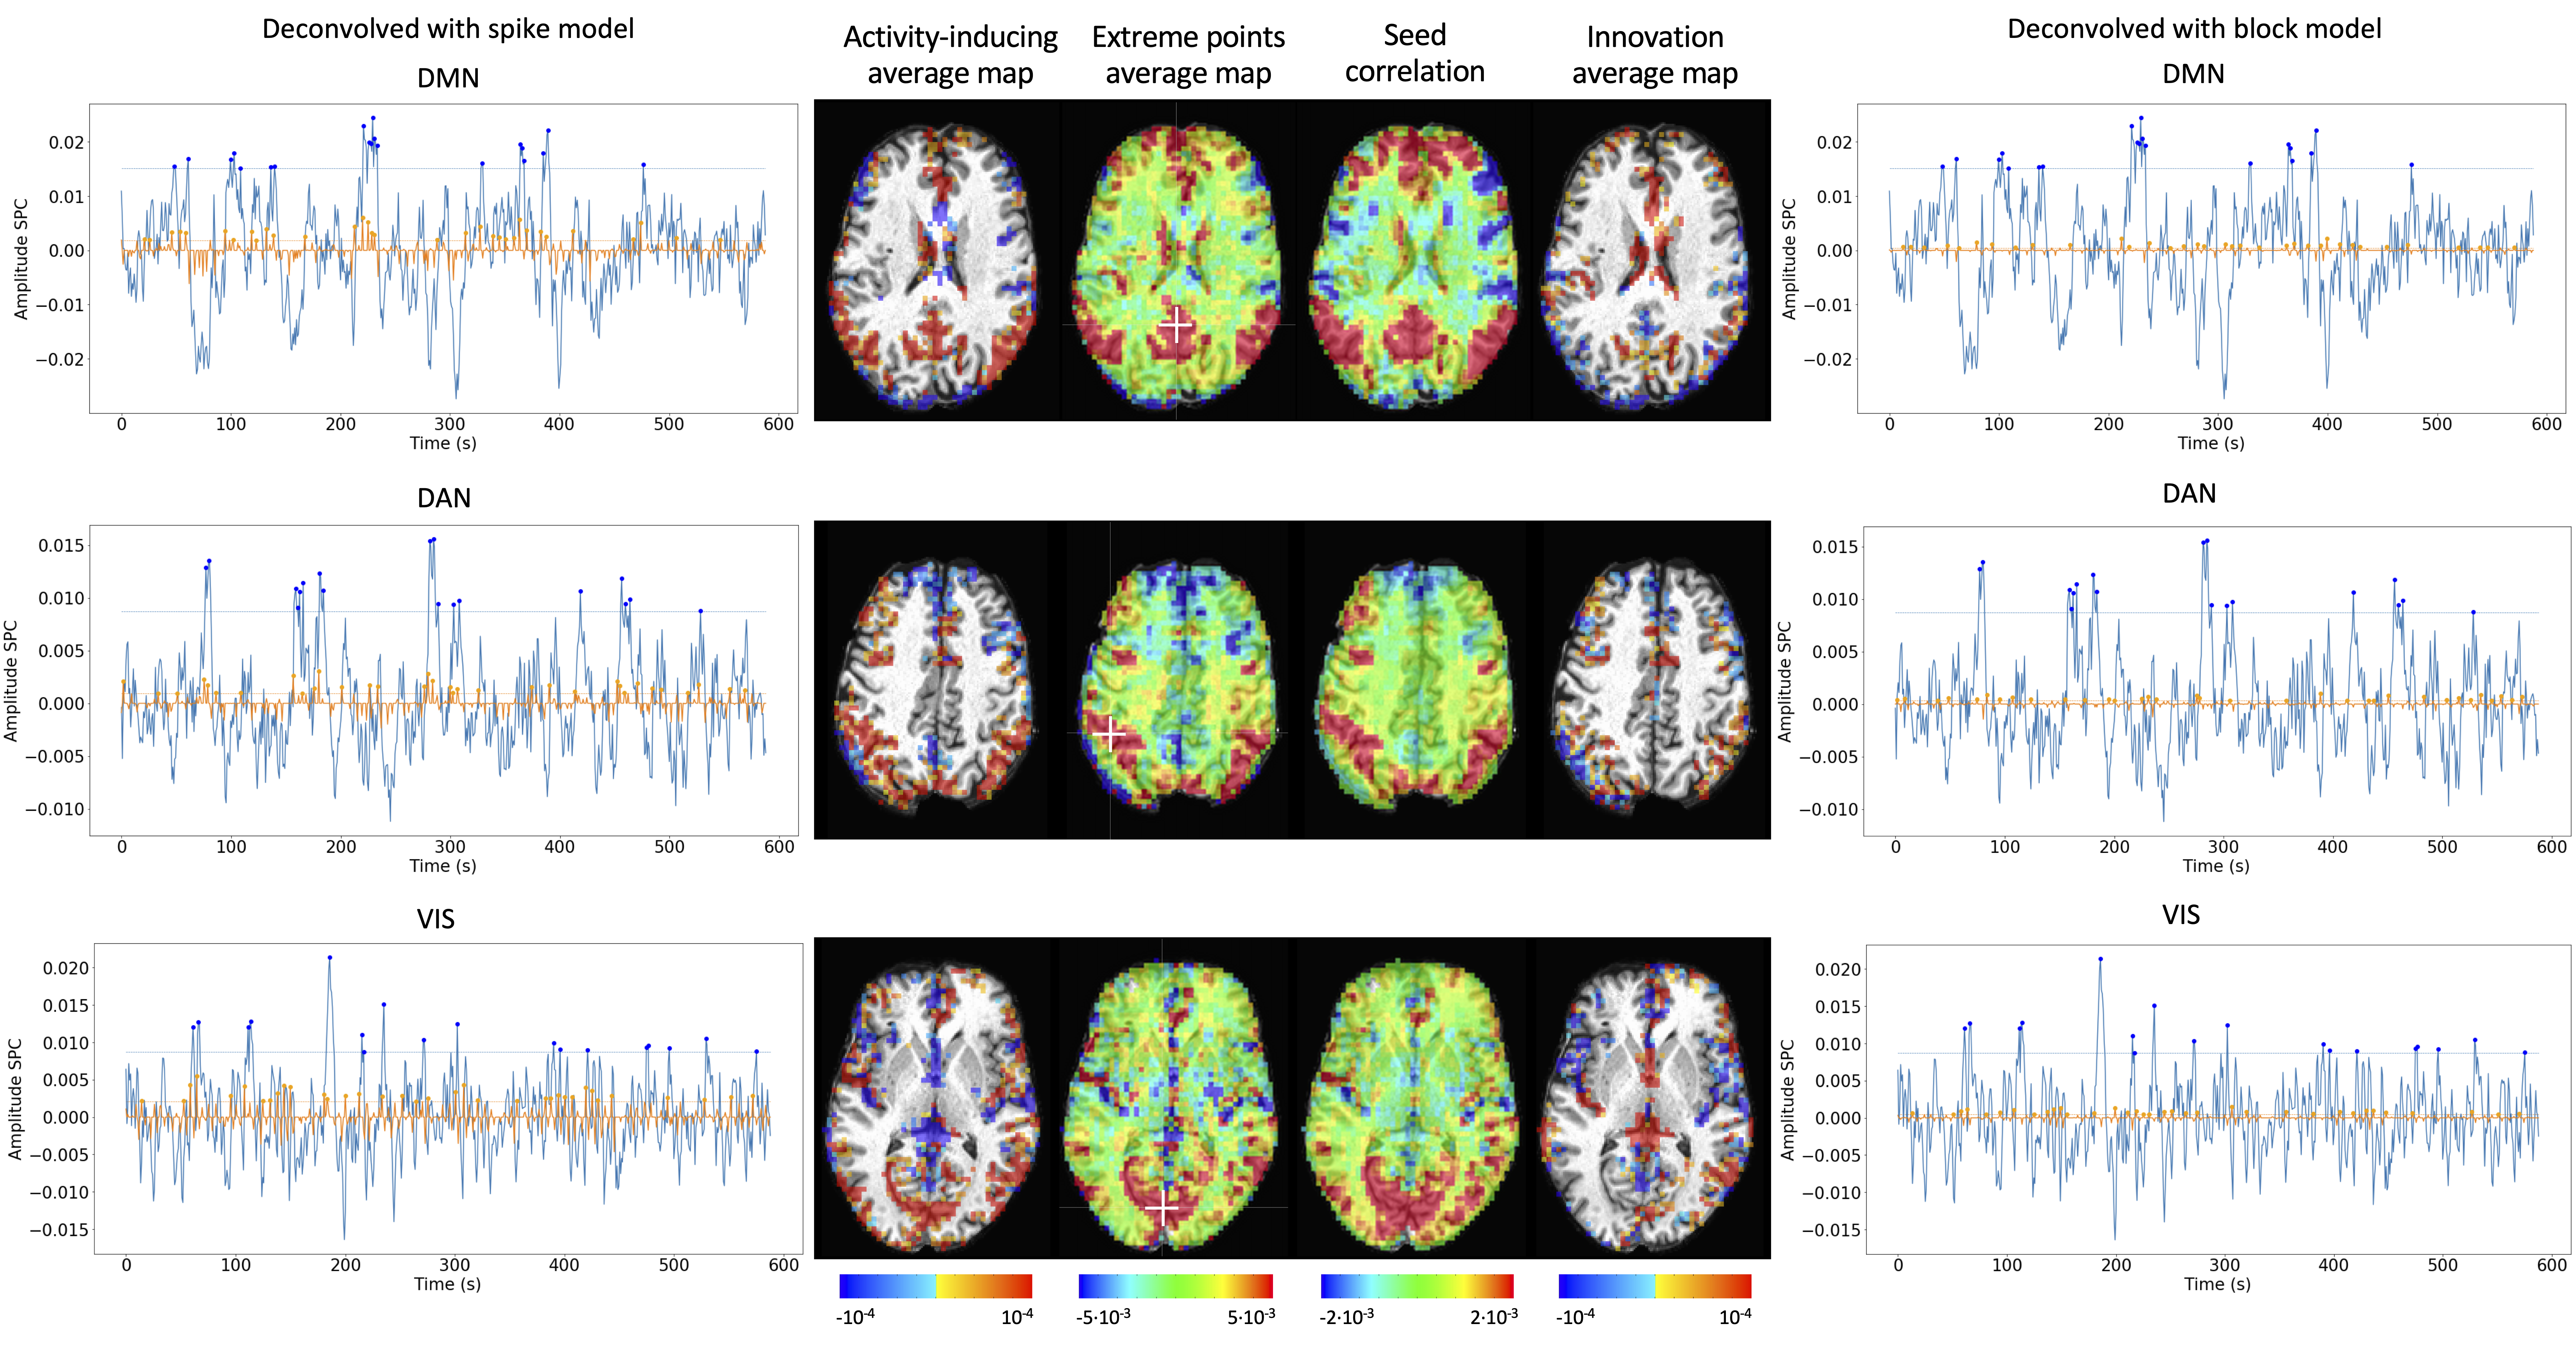
\includegraphics[width=\textwidth]{figures/supp_caps_mad.pdf}
    \end{center}
    \caption{CAPs MAD.}
\label{fig:caps_mad}
\end{figure*}

\end{document}